\documentclass{sig-alternate-ipsn13}

\begin{document}

\title{Device-free indoor localisation}
%
% You need the command \numberofauthors to handle the 'placement
% and alignment' of the authors beneath the title.
%
% For aesthetic reasons, we recommend 'three authors at a time'
% i.e. three 'name/affiliation blocks' be placed beneath the title.
%
% NOTE: You are NOT restricted in how many 'rows' of
% "name/affiliations" may appear. We just ask that you restrict
% the number of 'columns' to three.
%
% Because of the available 'opening page real-estate'
% we ask you to refrain from putting more than six authors
% (two rows with three columns) beneath the article title.
% More than six makes the first-page appear very cluttered indeed.
%
% Use the \alignauthor commands to handle the names
% and affiliations for an 'aesthetic maximum' of six authors.
% Add names, affiliations, addresses for
% the seventh etc. author(s) as the argument for the
% \additionalauthors command.
% These 'additional authors' will be output/set for you
% without further effort on your part as the last section in
% the body of your article BEFORE References or any Appendices.

% \numberofauthors{2} %  in this sample file, there are a *total*
% of EIGHT authors. SIX appear on the 'first-page' (for formatting
% reasons) and the remaining two appear in the \additionalauthors section.
%
% \author{\vspace{-2cm}
% You can go ahead and credit any number of authors here,
% e.g. one 'row of three' or two rows (consisting of one row of three
% and a second row of one, two or three).
%
% The command \alignauthor (no curly braces needed) should
% precede each author name, affiliation/snail-mail address and
% e-mail address. Additionally, tag each line of
% affiliation/address with \affaddr, and tag the
% e-mail address with \email.
%Markus~Matoni,
%         Michael~Krawez,
%         Gipsa~Joseph
%         and~Stephan~Sigg
% 1st. author
% \alignauthor
% 
% Markus Matoni, Michael Krawez, Gipsa Joseph\\
%        \affaddr{University of Goettingen}\\
% % 2nd. author
% % \and  % use '\and' if you need 'another row' of author names
% % 4th. author
% \alignauthor Stephan Sigg\\
%        \affaddr{University of Goettingen}\\
%        \affaddr{Networking Group}\\
%        \email{ssigg@gwdg.de}
% }
% There's nothing stopping you putting the seventh, eighth, etc.
% author on the opening page (as the 'third row') but we ask,
% for aesthetic reasons that you place these 'additional authors'
% in the \additional authors block, viz.
% Just remember to make sure that the TOTAL number of authors
% is the number that will appear on the first page PLUS the
% number that will appear in the \additionalauthors section.

\maketitle
\begin{abstract}
We present a device-free indoor localisation capable recognition system.
The system requires the installation of a single transmitter and receiver in each distinct room.
Rooms are clustered via non-overlapping frequencies. 
In-room localisation is achieved via learning of relative changes in the time-domain signal strength.
\end{abstract}


 \section{Extended abstract}
Localisation of non-cooperating individuals has been investigated for several years now.
High accuracy has been achieved, for instance, by radio tomography~\cite{RFSensing_Wilson_2009} as well as via RSS fingerprint maps~\cite{Pervasive_Seifeldin_2013}. 
Also, Zhang et al. could demonstrate a high accuracy of below 1m for the simultaneous tracking of five moving targets by isolating the LoS path between nodes~\cite{Pervasive_Zhang_2012}.
However, also from less complex, time-domain systems some localisation capabilities have been reported~\cite{Pervasive_Sigg_2012}.
% While the accuracy of the latter systems is naturally lower, also its installation and pre-processing cost is reduced.
This demo shows the potential of the localisation via time-domain signal strength features from pairs of software defined radio (SDR) nodes in limited range indoor scenarios.

\section{System description}
Our system employs pairs of transmit/receive software defined radio devices that continuously transmit an RF signal.\footnote{We employ USRP software defined radio nodes (http://www.ettus.com)}
Fluctuation in the relative time-domain signal strength is translated by the system to movement in various areas in a room.
In order to mitigate interference from transmitters in neighbouring rooms we employ a clustering approach in which each room represents a cell.
Devices operate on frequencies from 800MHz to 1.1 GHz and will be configured to non-overlapping frequencies in different rooms.
Signal streams will be processed for each device-pair separately and classification results are transmitted to a mobile device that then displays the detected location of individuals.
% This scenario is depicted in figure~\ref{figureScenario}.
% \begin{figure}
%  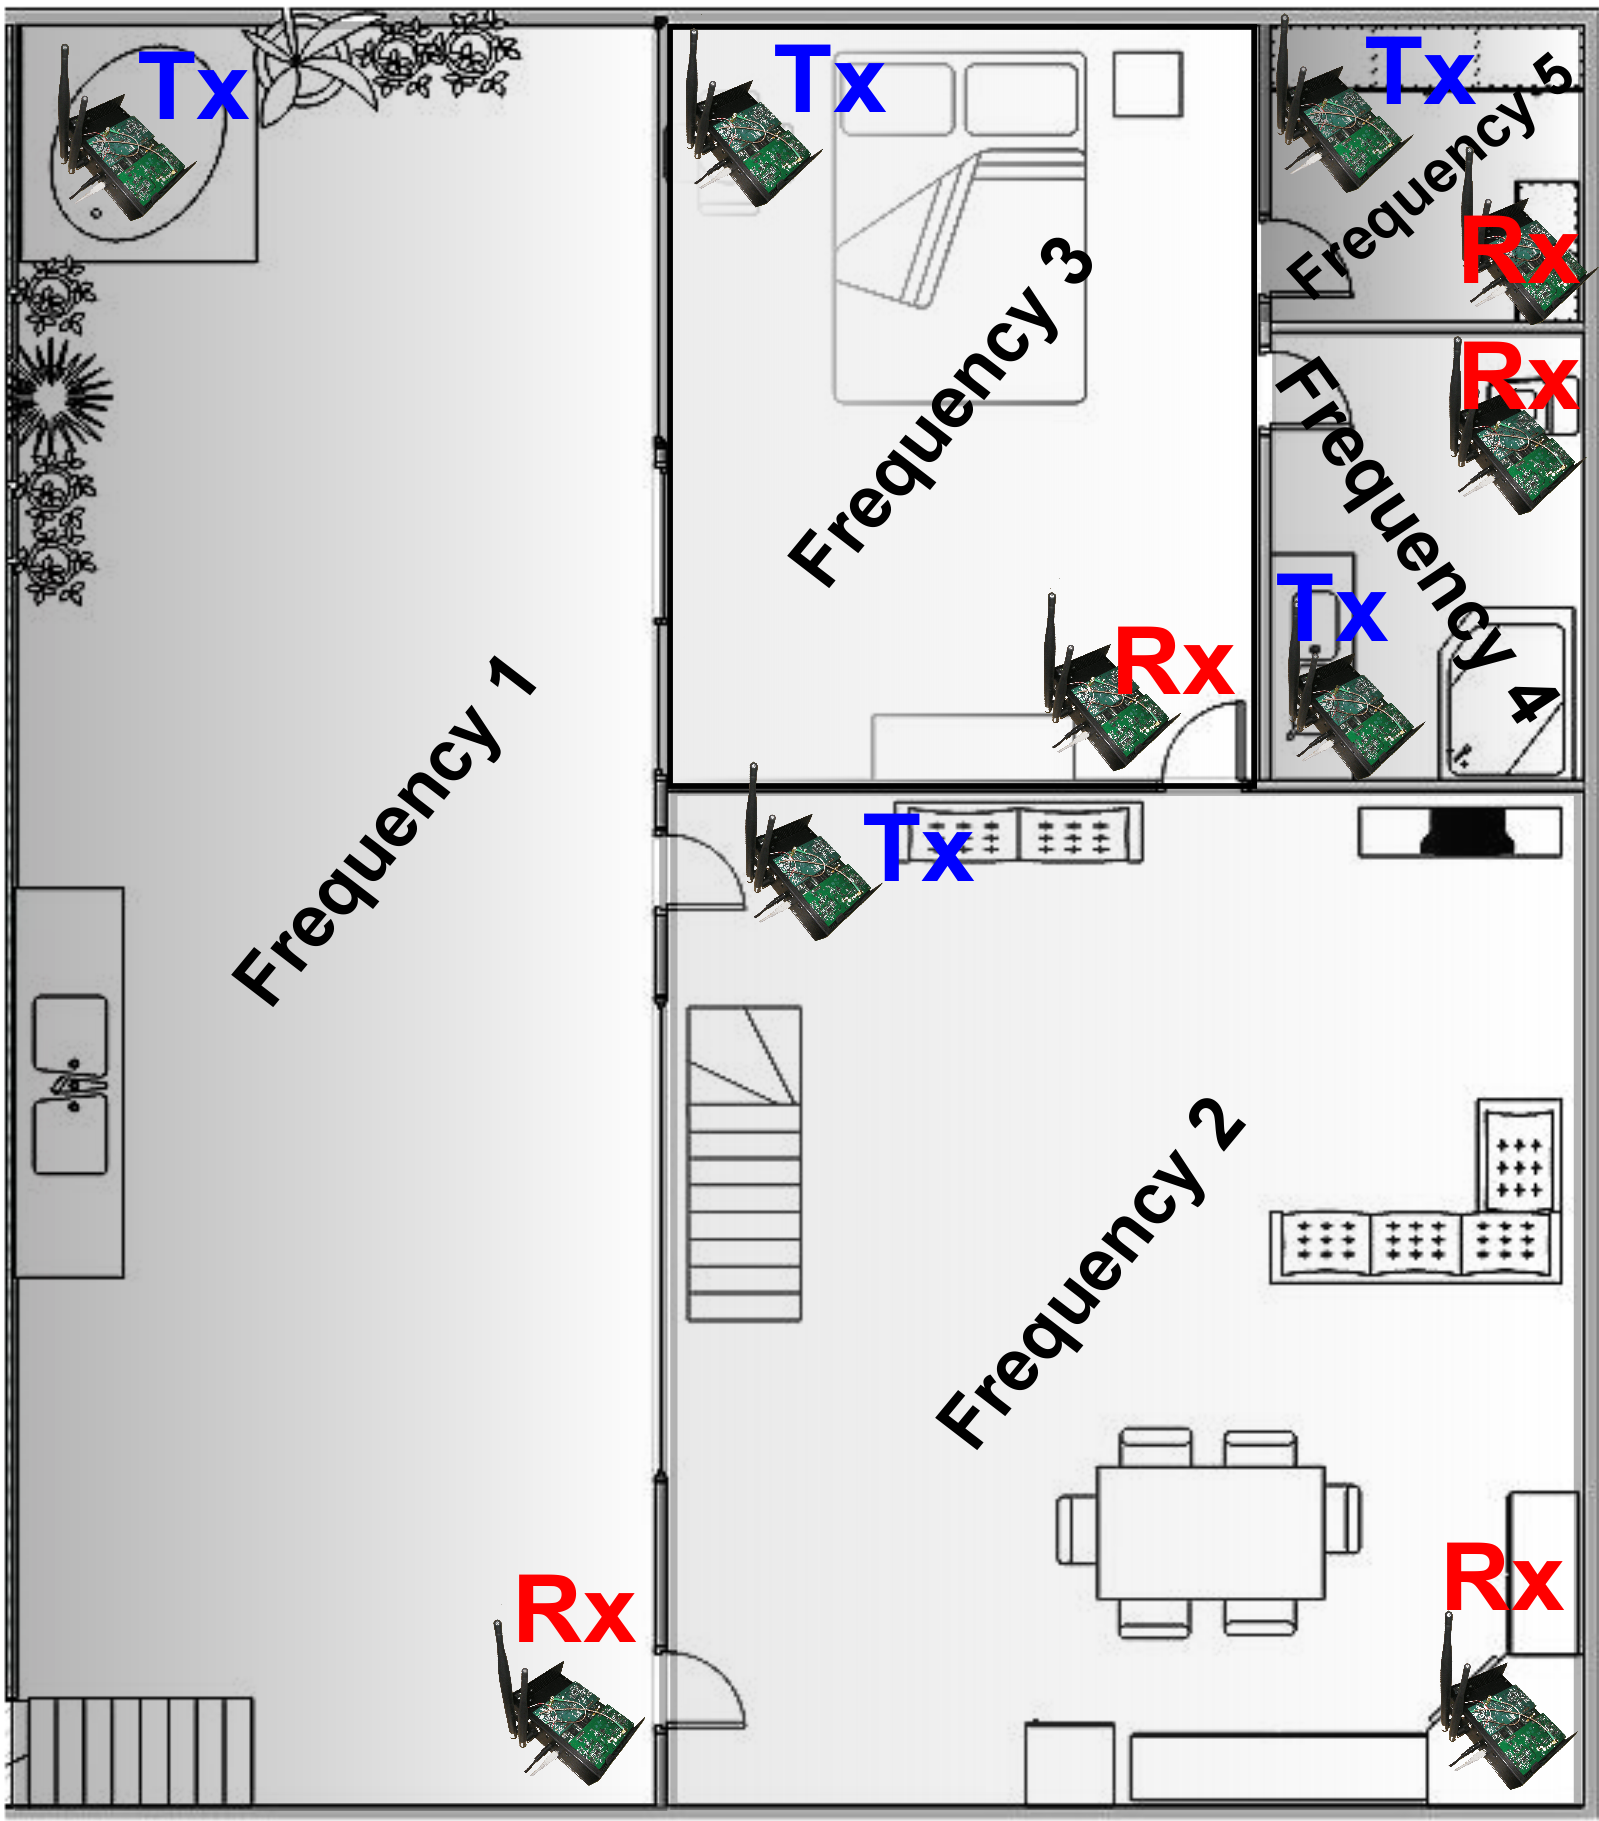
\includegraphics[width=\columnwidth, height=6cm]{Figures/sketch2.png}
%  \caption{Schematic illustration of a possible instrumentation of the system}
%  \label{figureScenario}
% \end{figure}
The fluctuation in the signal modulated to the wireless carrier is sampled at the receiver at 70Hz. 
Features are then calculated from this signal stream at the receiver.
In this system, we utilise the count of signal peaks within 10\%\ of the maximum, the mean difference between subsequent maxima, the count of zero crossings, %the standard deviation, 
the variance and the mean as features to classify activities.
This set of features is the result of a feature selection and manual feature reduction we conducted on a total of 17 features and their pair-wise combination. 
Since absolute signal strength might differ on consecutive days, relative signal-strength fluctuation is utilised. 
For this, all features are normalised to the mean signal strength experienced over a longer time period.

% Classification is then conducted by Decision tree, k-NN and Bayes classifiers.
% In the case that an activity is detected, this is transmitted to the mobile device where the activity is then displayed. 



%
% The following two commands are all you need in the
% initial runs of your .tex file to
% produce the bibliography for the citations in your paper.
\bibliographystyle{abbrv}
\bibliography{/home/stephan/Daten/Arbeit/Veroeffentlichungen/Literatur/Literatur_080128_v2_STS.bib}  % sigproc.bib is the name of the Bibliography in this case
% You must have a proper ".bib" file
%  and remember to run:
% latex bibtex latex latex
% to resolve all references
%
% ACM needs 'a single self-contained file'!
%
%APPENDICES are optional
%\balancecolumns
% \appendix
%Appendix A

% Appendix goes here.

% That's all folks!
\end{document}
